\section{Stellar evolution}\label{sec:stellar_evolution}

The stellar evolution calculations in this work are performed using the normal AMUSE parameters for MESA, with solar metallicity as the input.
MESA allows me to track the independent evolution of the triple system components and obtain estimations of their properties at the beginning of \ac{rlof}. In this work, I allow the three stars of the system to evolve until the tertiary overfill it's Roche lobe, such as $R_{stop} = 1.1 \times R_{L}$, see \cref{eq:roche_lobe}. The consequence of this choice will be discussed in detail in \cref{simulations}.

By the time the outer star approaches the radius of its Roche lobe, all three stars have lost some mass via stellar winds, while the tertiary's radius is much bigger than when it was formed. In order to accurately evaluate the Roche lobe sizes, I need to estimate the masses of the stars at the \ac{rlof} moment. Unfortunately, $\xi$ Tau's age is not known, but mass-loss via winds during the main sequence is expected to be unimportant for low- and intermediate- mass stars, see \cref{sub:winds}.

Despite that, I track the evolution of the tertiary's mass and radius profile. As expected, radiation-driven mass-loss proved negligible in this mass regime. For cold winds, I utilize Reimer's, see \cref{eq:reimer}, and Blocker's, see \cref{eq:blocker}, mass-loss prescriptions using commonly used scaling factors of $\eta = 0.5$ and $\eta = 0.1$, respectively. 
\begin{figure}[H]
    \centering
    \begin{subfigure}{.5\textwidth}
    \centering
    \includegraphics[width=0.9\textwidth]{Thesis/graphs/giant_1-1mass_loss.pdf}
    \label{fig:mass_loss}
    \end{subfigure}%
    \begin{subfigure}{.5\textwidth}
    \centering
    \includegraphics[width=0.9\textwidth]{Thesis/graphs/giant_1-1radius.pdf}
    \label{fig:radius_profile}
    \end{subfigure}
    \caption{ Mass and radius evolution of a 5.5 M$_{\odot}$ star at solar metallicity until \ac{rlof}. \ac{zams} and \ac{tams} are noted by black circles, while the start and end of helium burning by black squares. I create the stellar evolution models using MESA \citep{paxton2010modules,paxton2013modules,paxton2015modules,paxton2019modules}.}
\end{figure}
The tertiary loses less than $1\%$ of its 
initial mass, while the expected mass-loss from the binary components is even smaller, because less massive, and thus less luminus, stars will have weaker winds. As a result, I do not correct for mass-loss and use the parameters listed in  \cref{tab:system_orbit_param}.  

At this point, I also assume that the mass lost through winds has no effect on the stars. This assumption would be false in the case of more massive stars. As mass escapes from the star's surface, it carries angular momentum and can change the inner and outer orbital parameters. Furthermore, some of the escaped mass can be accreted, complicating the evolution of the two orbits even further. Given the small amount of mass loss, the aforementioned assumption is safe in this case.

In \cref{fig:HR_ROLF}, I present the evolution of the tertiary on the \ac{hrd} until the moment of \ac{rlof} and in \cref{tab:tertiary_param_ROLF} I summarize the tertiary's important stellar parameters. 
\begin{figure}[H]
    \centering
    \includegraphics[width=0.9\textwidth]{Thesis/graphs/HR_1-1ROLF.pdf}
    \caption{Evolution of 5.5 M$_{\odot}$ at solar metallicity until the moment of \ac{rlof}. \ac{zams} and \ac{tams} are noted by black circles, while the start and end of helium burning by black squares. The evolutionary phases are categorized in different colors similar to \cref{fig:HR_evolution}. I calculate the track using MESA \citep{paxton2010modules,paxton2013modules,paxton2015modules,paxton2019modules}. The dashed lines show lines of constant radii by means of the Stefan–Boltzmann law.}
    \label{fig:HR_ROLF}
\end{figure}
\begin{table}[H]
    \centering
    \begin{tabular}{| c | c |}
       Parameter & Value \\
       \hline 
       M$_{RLOF}$ & 5.5 (M$_{\odot}$) \\
       R$_{RLOF}$ & 91.36 (R$_{\odot}$) \\
       L$_{RLOF}$ & 2262 (L$_{\odot}$) \\
       t$_{RLOF}$ & 82.36 (Myr) 
    \end{tabular}
    \caption{ $\xi$ Tau parameters at the beginning of \ac{rlof}. From top to bottom the tertiary's mass, radius, luminosity and age.}
    \label{tab:tertiary_param_ROLF}
\end{table}
The tertiary overflows its Roche lobe during the early \ac{agb} phase, see \cref{fig:HR_ROLF}, after helium exhaustion, leading to a type C mass transfer. \cref{fig:HR_ROLF} shows that when \ac{rlof} occurs, $T_{eff} < 10^{3.7} K$. For such low temperature the envelope's opacity can be high enough so that that the later will be unstable against convection, see \cref{sec:convection}. 

I present a Kippenhahn diagram of the tertiary, see \cref{fig:kippen_plot}. This diagram displays the structural evolution of the star from the core to the photosphere. The vertical axis represents the position within the star in terms of enclosed mass and the horizontal axis represents the number of the models, which are translated to stellar age (hence the x-axis is not linear). In this diagram, one can see how different regions are discerned: The white parts are the radiative regions, the stripped parts represent the convective regions, and the variation of the color represent the intensity of the energy generation at various regions in arbitrary units. Darker color indicate that more energy is produced.
\begin{figure}[H]
    \centering
    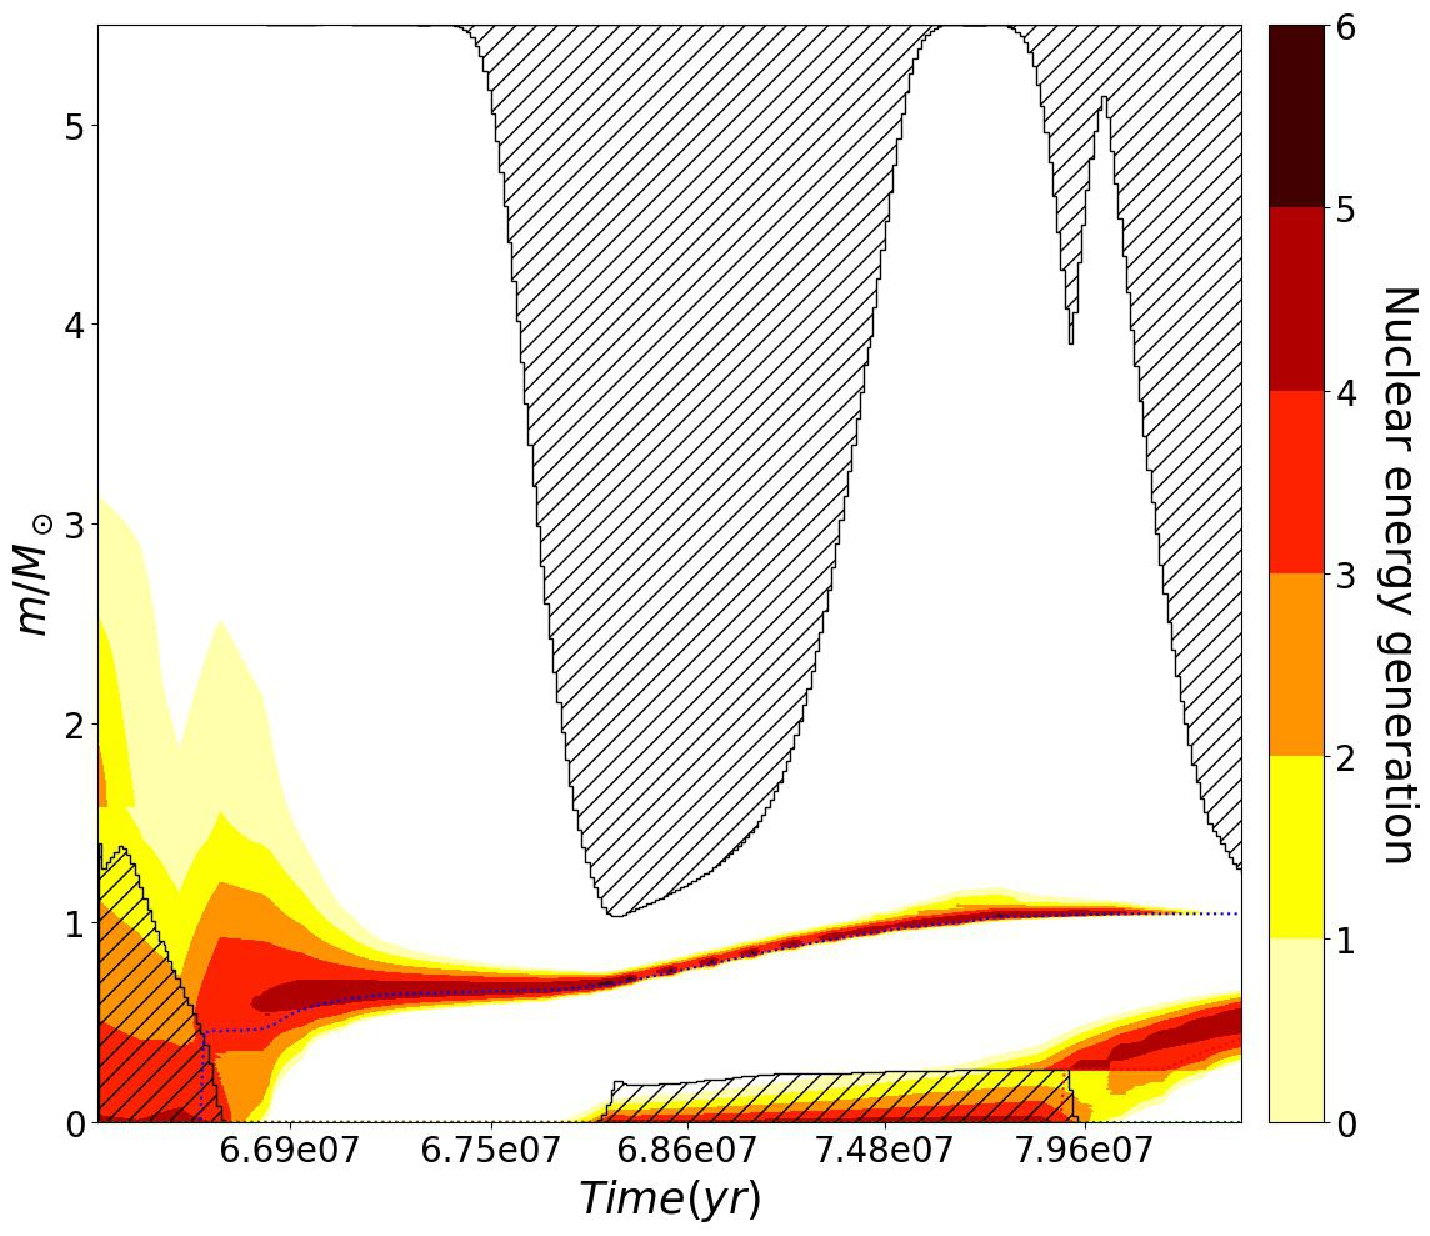
\includegraphics[width=0.9\textwidth]{Thesis/graphs/Kippen_ROLF_Schw.pdf}
    \caption{Kippenhahn diagram of $\xi$ Tau outer component until the onset of \ac{rlof} using Schwarzwild criterion, see \cref{eq:Schwarzwild_criterion}. The vertical axis represents the position within the star in terms of enclosed mass and the horizontal axis represents the number of the models which are translated to stellar age. The white parts are radiative regions, the stripped parts represent convective regions, and the variation of the color represent the intensity of the energy generation at various regions in arbitrary units. Darker color indicate that more energy is produced. I create the graph using MESA \citep{paxton2010modules,paxton2013modules,paxton2015modules,paxton2019modules}.}
    \label{fig:kippen_plot}
\end{figure}
\cref{fig:kippen_plot} shows that at the moment of \ac{rlof}, the convective envelope has penetrated deep inside the star close to the actual core. Hence, convective mixing is expected to enrich the outer layers of the star with metal-rich material. Additionally, in this case, convection defines the mechanical structure of the envelope. This is critical for the 3D hydrodynamical model and it is discussed in detail in \cref{sec:1D_to_3D}. 

Given the parameters in \cref{tab:tertiary_param_ROLF}, I also calculate the relevant characteristic timescales of the tertiary, see \cref{sec:timescales}, which are listed in \cref{tab:tertiary_timescale_ROLF}.
\begin{table}[H]
    \centering
    \begin{tabular}{| c | c |}
       Timescale & Duration \\
       \hline
       $t_{dyn}$ & 4.85 day\\
       $t_{th}$ & 4585.78 yr 
    \end{tabular}
    \caption{ Tertiary timescales at the beginning of \ac{rlof}.}
    \label{tab:tertiary_timescale_ROLF}
\end{table}
\begin{comment}
In \cref{tab:system_orbit_param_ROLF} I summarize the important parameters of the system at the moment of \ac{rlof}. 
\begin{table}[H]
    \begin{adjustbox}{width=1\textwidth}
    \small
    \centering
    \begin{tabular}{| c c c c c c c c c c|}
       M$_1$ (M$_{\odot}$) & 
       M$_2$ (M$_{\odot}$) &
       M$_3$ (M$_{\odot}$) & $\alpha_{in}$ (au) &
       $\alpha_{out}$ (au) &
       $\epsilon_{in}$ &
       $\epsilon_{out}$ &
       $R_{RLOF}$ (au) &
       $t_{RLOF}$ (Myr) &
       $M_{RLOF}$  (M$_{\odot}$) \\
       \hline
       3.2 & 3.1 & 5.5 & 0.133 & 1.24 & 0.0 & 0.15 & 0.423 & 82.36 & 5.5
    \end{tabular}
    \end{adjustbox}
    \caption{ Orbital parameters of $\xi$ Tau system at the beginning of \ac{rlof}}
    \label{tab:system_orbit_param_ROLF}
\end{table}
Given these parameters, I also calculate the relevant characteristic timescales of the tertiary, which are listed in \cref{tab:tertiary_timescale_ROLF}.
\begin{table}[H]
    \centering
    \begin{tabular}{| c | c |}
       Timescale & Duration \\
       \hline
       $t_{dyn}$ & 4.85 day\\
       $t_{th}$ & 4585.78 yr 
    \end{tabular}
    \caption{ Tertiary timescales at the beginning of \ac{rlof}.}
    \label{tab:tertiary_timescale_ROLF}
\end{table}
\end{comment}
Note that the default parameters of MESA withing AMUSE do not include overshooting. However, I perform one test taking into account overshooting with $f=0.016$ \citep{herwig2000evolution}. On the one hand, the \ac{ms} lifetime extends, \ac{rlof} occurs $~10Myr$ later in the evolution, while the stellar core is more massive. On the other hand, the impact on the structure of the envelope's outer layers at the moment of \ac{rlof} is negligible. This is the region of highest interest for my mass transfer simulations, thus I proceed with models without overshooting. Nevertheless, it is worth mentioning that for $f=0.016$, \ac{rlof} occurs before helium exhaustion leading to a type B mass transfer.
